\begin{figure}[htbp]
\centering
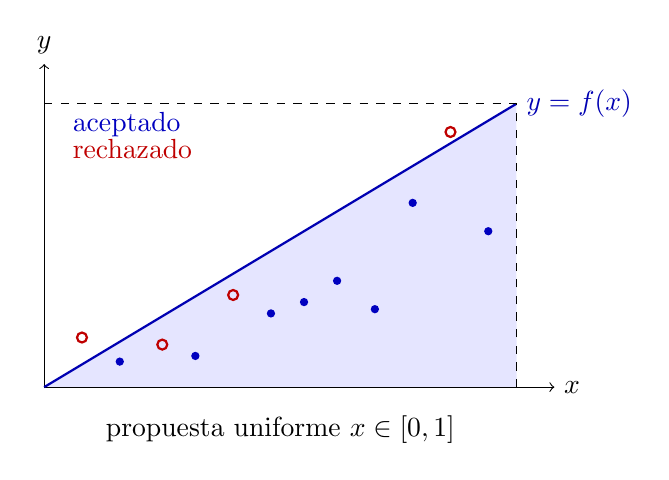
\begin{tikzpicture}[x=6cm,y=1.8cm]
  \fill[blue!10] (0,0) -- plot[domain=0:1,samples=60] (\x,{2*\x}) -- (1,0) -- cycle;
  \draw[->] (0,0) -- (1.08,0) node[right] {$x$};
  \draw[->] (0,0) -- (0,2.28) node[above] {$y$};
  \draw[thick,blue!70!black,domain=0:1,samples=60] plot (\x,{2*\x})
    node[right] {$y=f(x)$};
  \draw[dashed] (1,0) -- (1,2);
  \draw[dashed] (0,2) -- (1,2);
  \foreach \x/\y in {0.16/0.18,0.32/0.22,0.48/0.52,0.55/0.60,
                      0.62/0.75,0.70/0.55,0.78/1.30,0.94/1.10}
    \fill[blue!75!black] (\x,\y) circle (1.5pt);
  \foreach \x/\y in {0.08/0.35,0.25/0.30,0.40/0.65,0.86/1.80}
    \draw[red!75!black,thick] (\x,\y) circle (1.8pt);
  \node[blue!75!black,anchor=west] at (0.04,1.85) {aceptado};
  \node[red!75!black,anchor=west] at (0.04,1.68) {rechazado};
  \node[below] at (0.5,-0.13) {propuesta uniforme $x\in[0,1]$};
\end{tikzpicture}
\caption{Cada punto se propone uniformemente en el rectángulo $[0,1]\times[0,2]$. Se conserva si queda bajo $f(x)=2x$. Los puntos son ilustrativos.}\label{fig:puntos}
\end{figure}